\section{Man-in-the-Middle Attack}
\subsection{Activity}

\noindent {\bf{Bước 1:}} Khởi động Windows Server. Thử sử dụng trình duyệt truy cập internet để xác minh kết nối.

\begin{figure}[!htb]
    \centering
    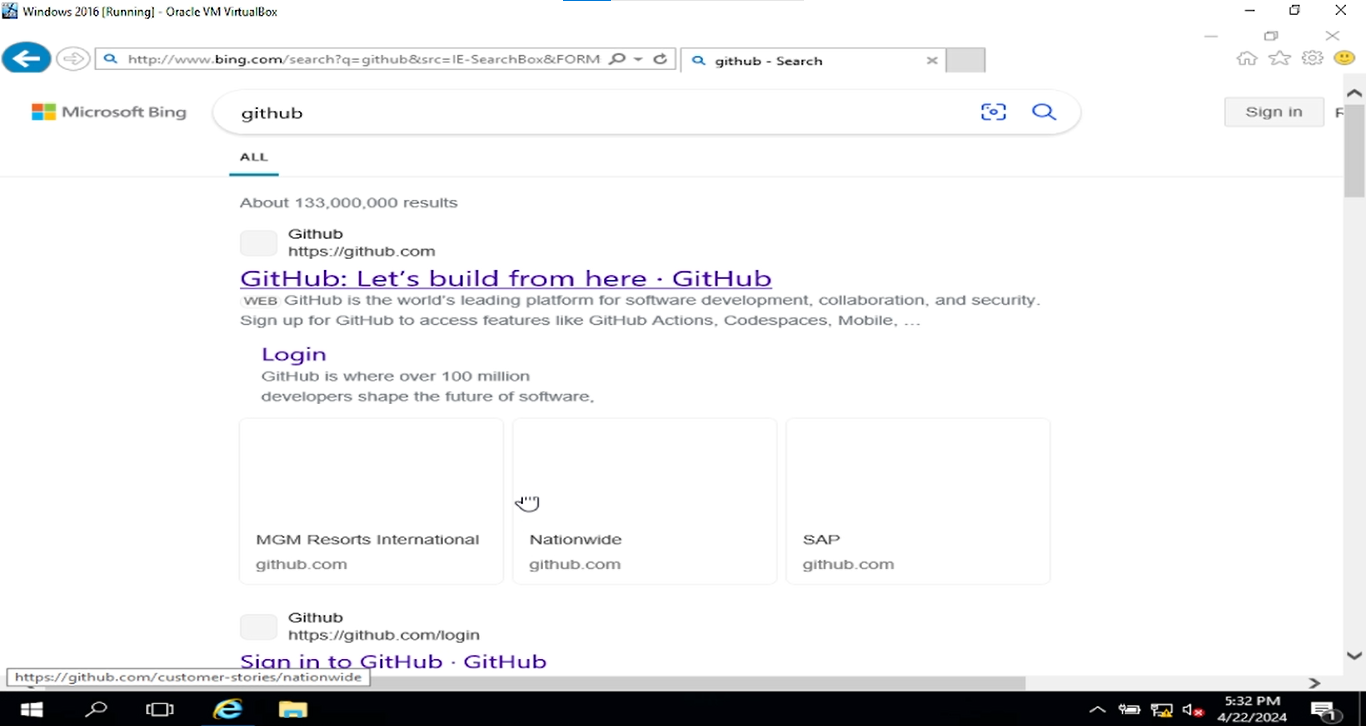
\includegraphics[width=1\linewidth]{figure//chapter5//lab5_4/verify.png}
    \caption{Xác minh kết nối khi search github trên google}
    \label{fig:enter-label}
\end{figure}

\noindent {\bf{Bước 2:}} Sử dụng Kali Linux VM và ping tới Windows Server.

\begin{figure}[!htb]
    \centering
    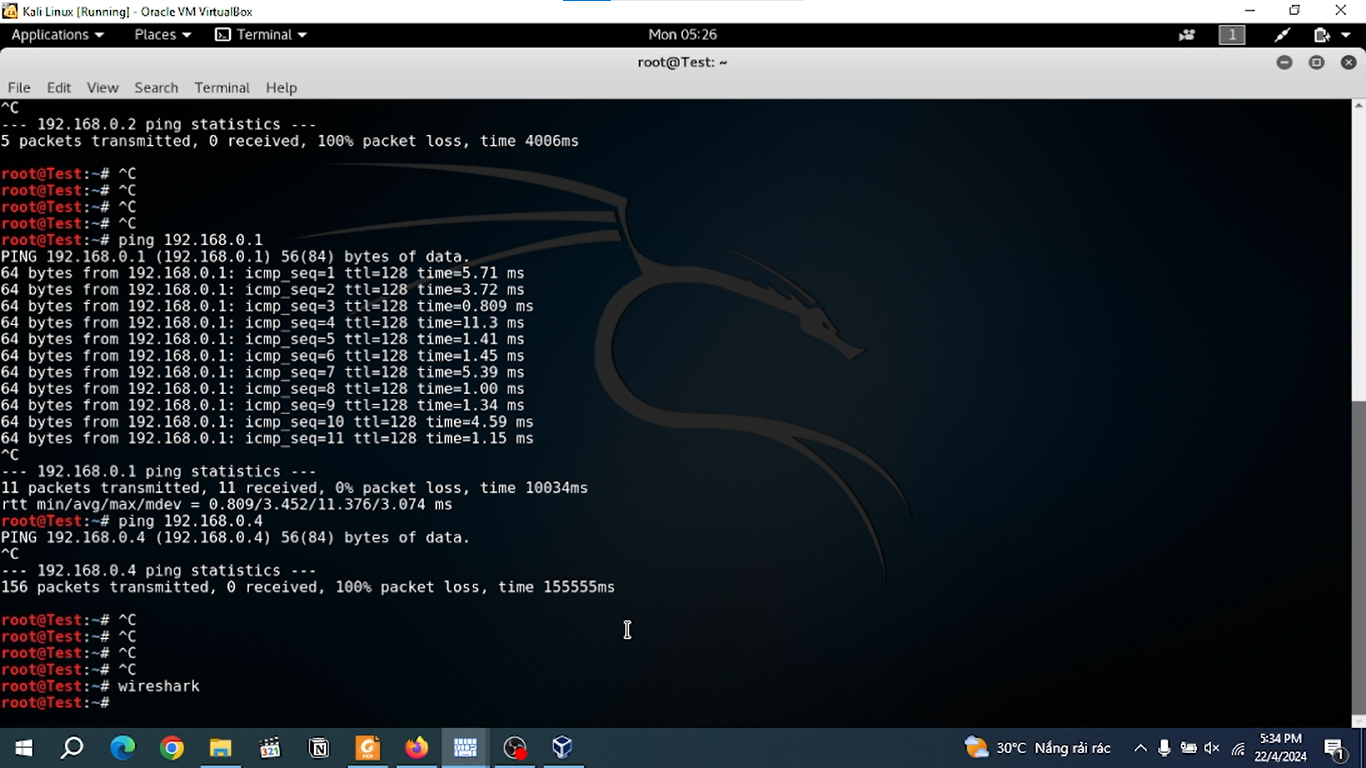
\includegraphics[width=1\linewidth]{figure//chapter5//lab5_4/verify_kali.png}
    \caption{Xác minh thông qua ping từ Kali Linux VM}
    \label{fig:enter-label}
\end{figure}

\newpage

\noindent {\bf{Bước 3:}} Vào \textbf{Application > Sniffing/Spoofing > Network Sniffers > ettercap-graphical}. Ở \textbf{Sniff} chọn \textbf{Unified Sniffing}. Sau đó, vào meny \textbf{Hosts}, thực hiện \textbf{Scan for hosts} và hiện \textbf{Hosts List} tương tự như ở phần 3. Để tiện sử dụng, ta sẽ chuyển các địa chỉ về 10.0.2.x mặc định của NAT Network.

\begin{figure}[!htb]
    \centering
    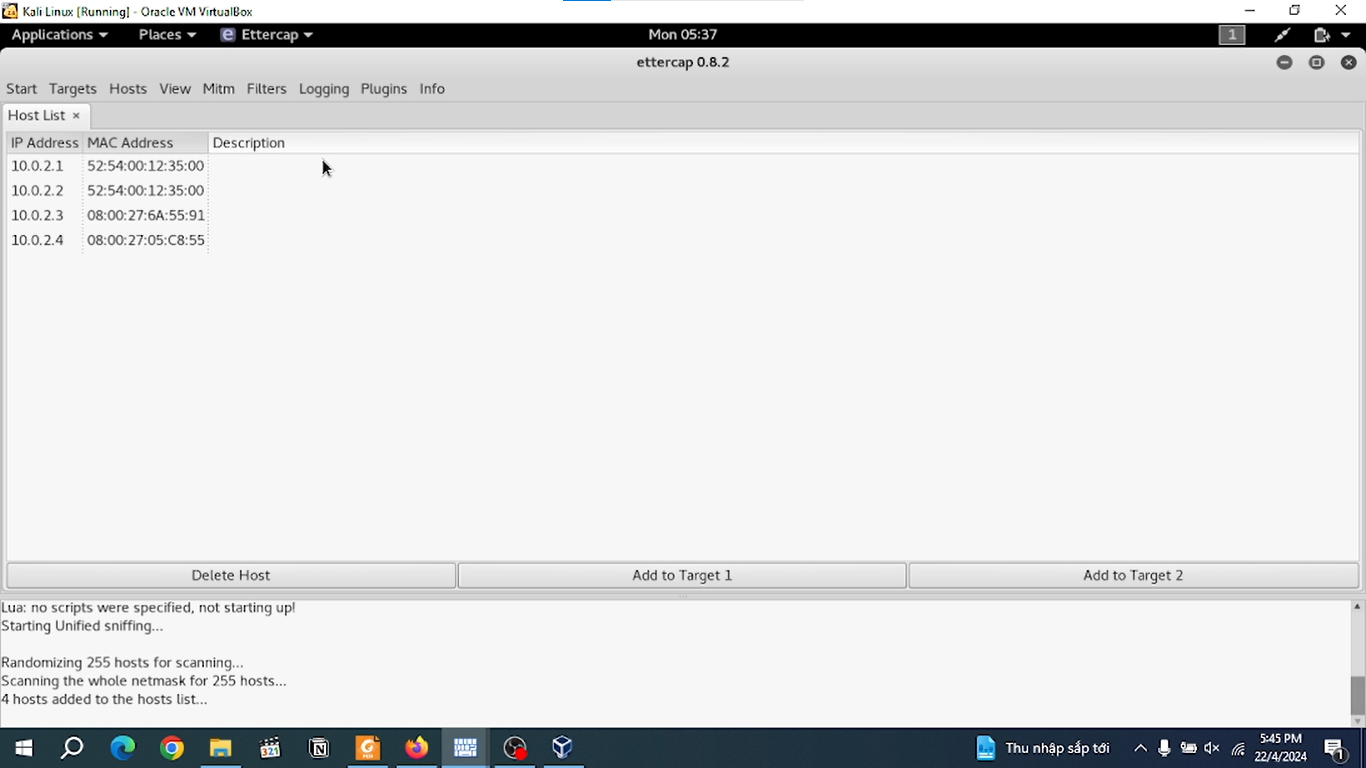
\includegraphics[width=1\linewidth]{figure//chapter5//lab5_4/host_list.png}
    \caption{Hosts List trong Ettercap-Graphical}
    \label{fig:enter-label}
\end{figure}

\noindent {\bf{Bước 4:}} Chọn 2 địa chỉ IP tương ứng với Windows Server và Windows 10 và lần lượt chọn \textbf{Add to Target 1} và \textbf{Add to Target 2}. Sau đó \textbf{Start sniffing}.

\begin{figure}[!htb]
    \centering
    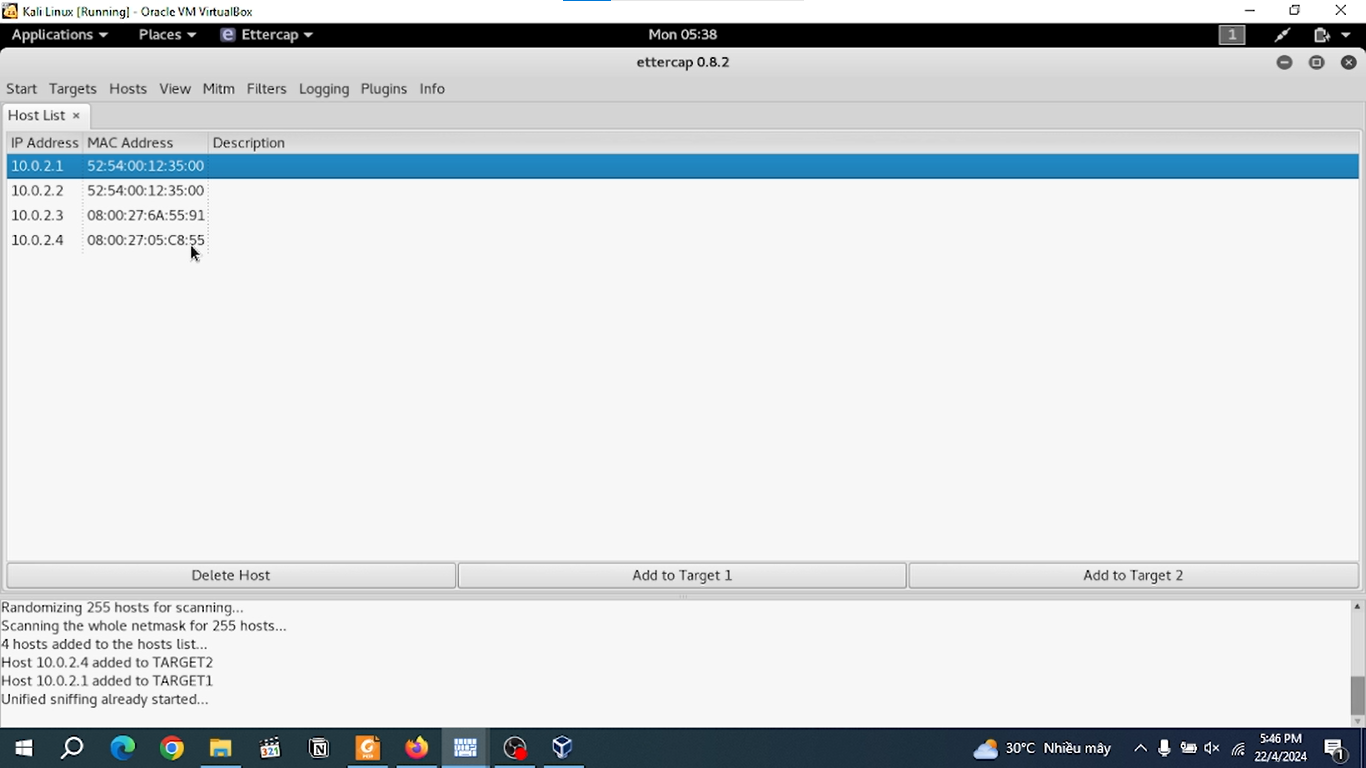
\includegraphics[width=0.95\linewidth]{figure//chapter5//lab5_4/start_sniffing.png}
    \caption{Start sniffing}
    \label{fig:enter-label}
\end{figure}

\newpage

\noindent {\bf{Bước 5:}} Ở menu \textbf{Mitm}, chọn \textbf{ARP Poisoning} rồi chọn \textbf{Sniff remote connections}. 

\begin{figure}[!htb]
    \centering
    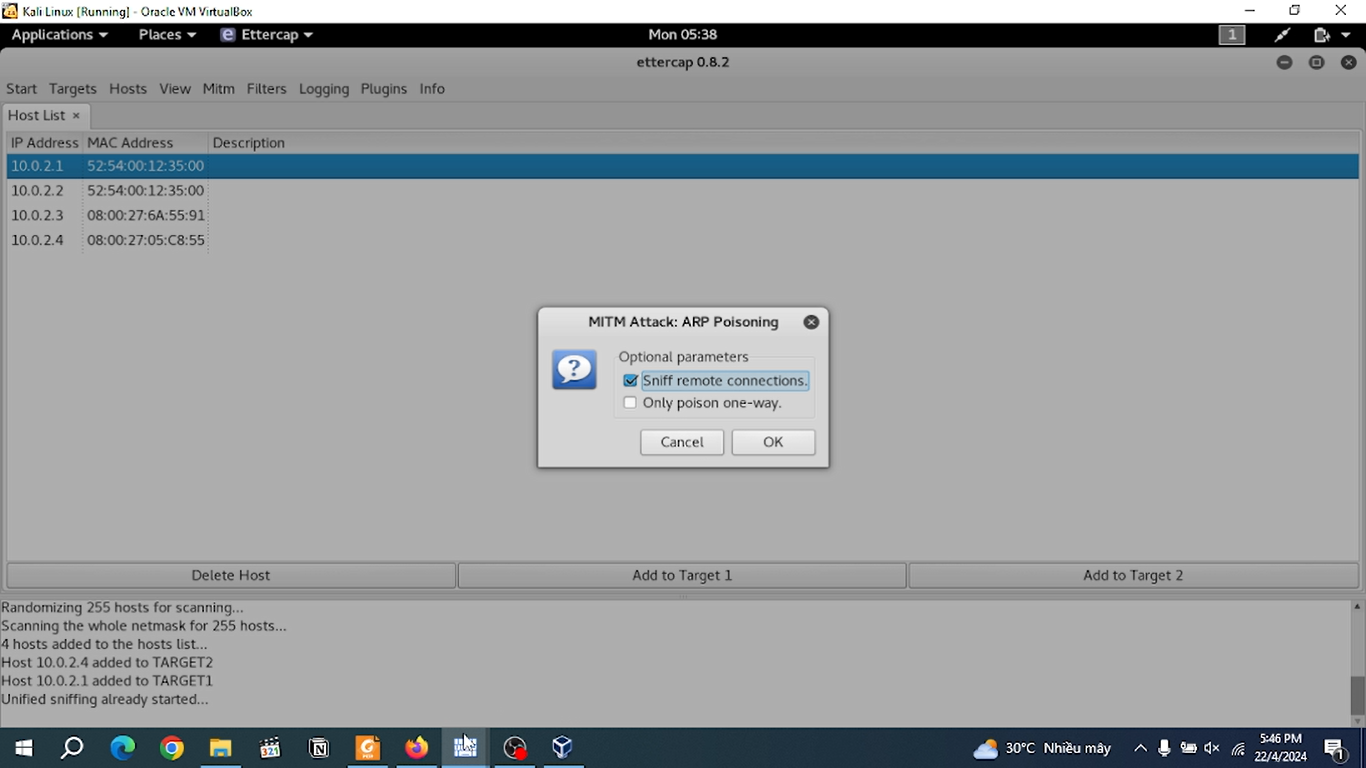
\includegraphics[width=1\linewidth]{figure//chapter5//lab5_4/mitm.png}
    \caption{Mitm configure}
    \label{fig:enter-label}
\end{figure}

\noindent {\bf{Bước 6:}} Vào \textbf{Plugins}, chọn \textbf{Manage the plugins}. Chọn \textbf{remote\_browser}.

\begin{figure}[!htb]
    \centering
    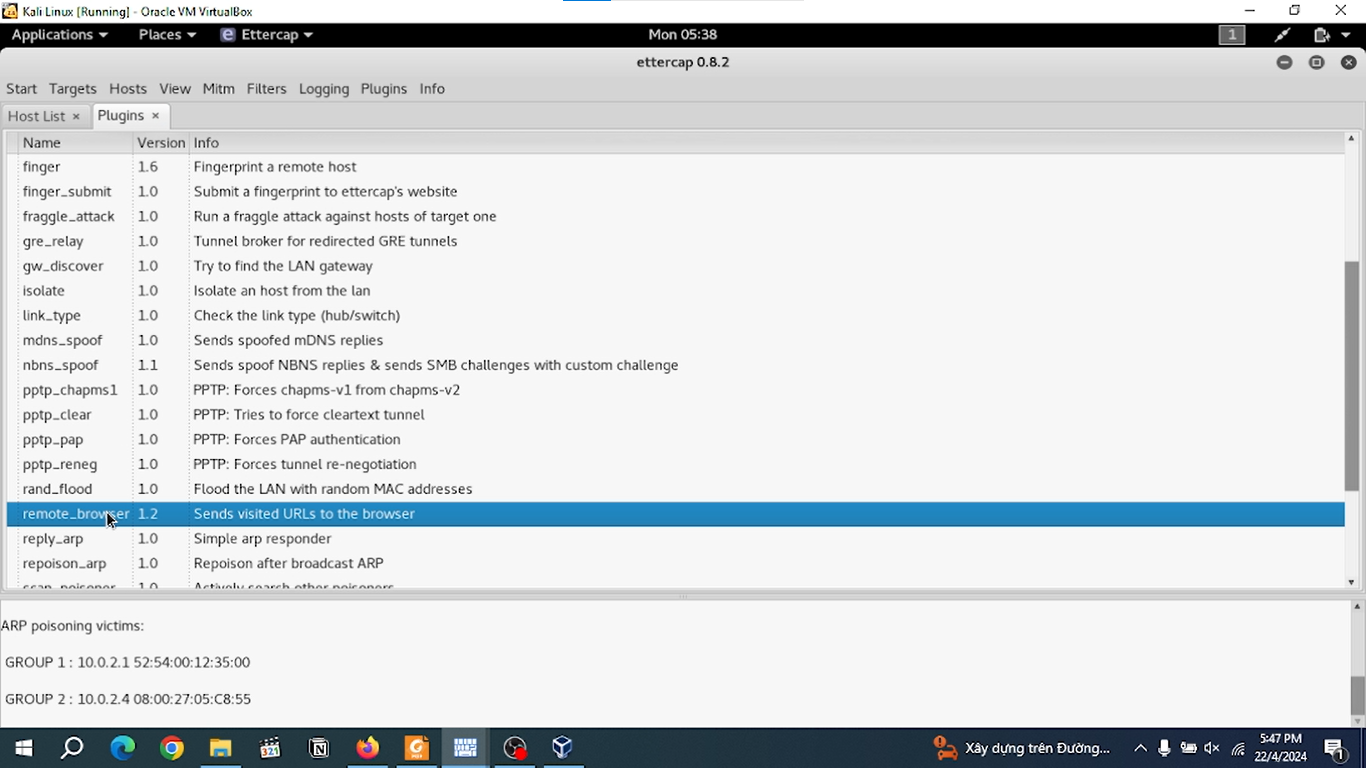
\includegraphics[width=1\linewidth]{figure//chapter5//lab5_4/remote_browser.png}
    \caption{Chọn remote\_browser plugin}
    \label{fig:enter-label}
\end{figure}

\newpage

\noindent {\bf{Bước 7:}} Ở Windows Server, vào \textbf{www.google.com}. Sau đó thông báo sẽ hiện ở ettercap.

\begin{figure}[!htb]
    \centering
    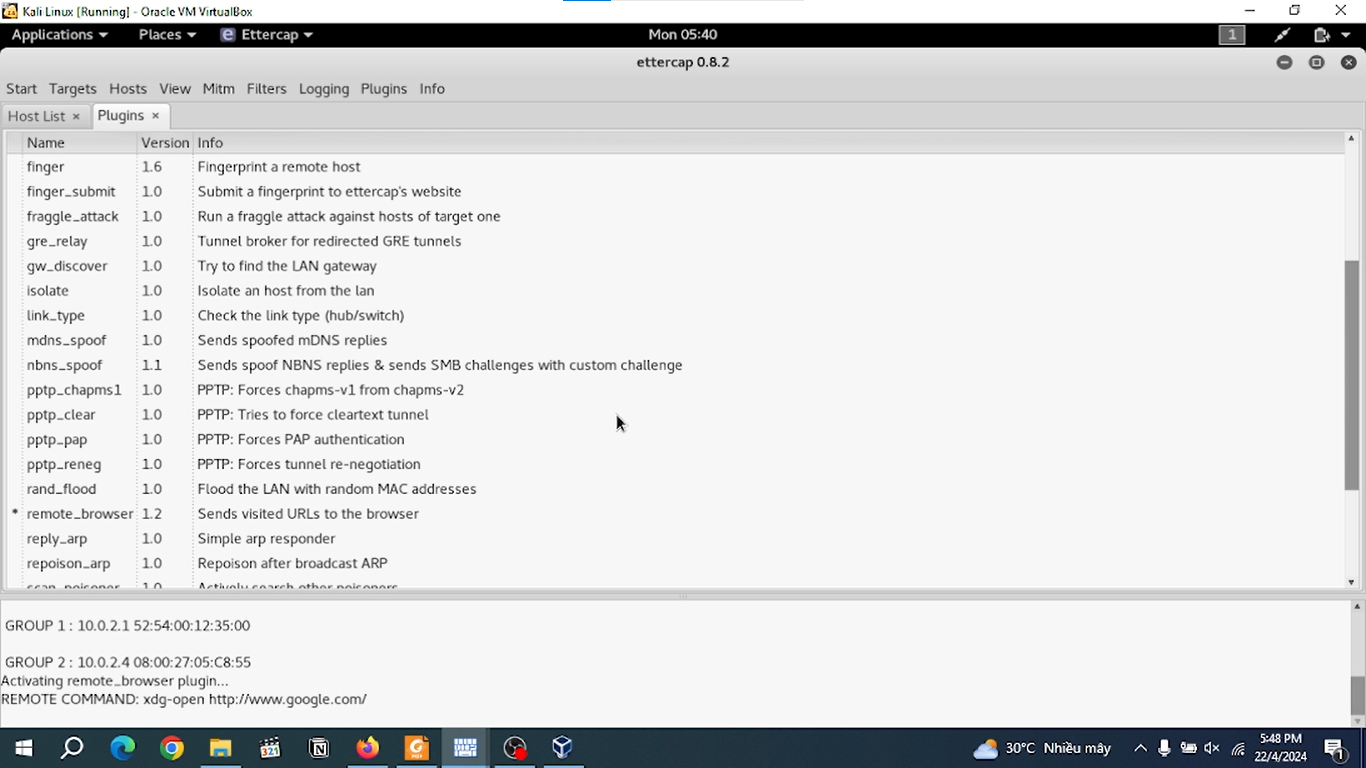
\includegraphics[width=1\linewidth]{figure//chapter5//lab5_4/result_searching_google.png}
    \caption{Kết quả khi tìm google}
    \label{fig:enter-label}
\end{figure}

\noindent {\bf{Bước 8:}} Sau đó, thử truy cập \textbf{www.yahoo.com} thì sẽ thấy rằng không thể tìm được. Chỉ sau khi thực hiện lệnh \textbf{arp -d *} để xoá cache của arp thì mới cho tế truy cập được.

\begin{figure}[!htb]
    \centering
    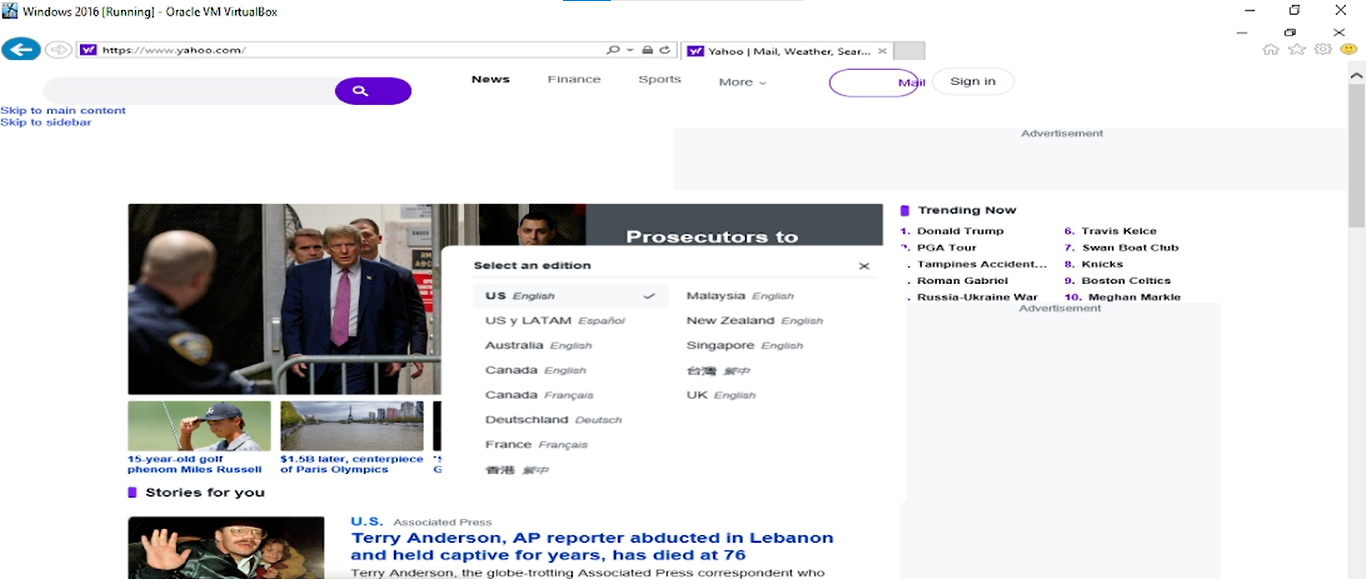
\includegraphics[width=1\linewidth]{figure//chapter5//lab5_4/result_search_yahoo.png}
    \caption{Kết quả khi tìm yahoo sau khi thực hiện arp -d *}
    \label{fig:enter-label}
\end{figure}

\newpage

\subsection{Review Questions}

\noindent Câu 1:

\noindent Câu 2: Default settings get restored.

\noindent Câu 3: 

A: An analysis of the network layer headers would indicate that Server has communicating directly with the internet.

C: An analysis of the network layer headers would indicate that Server has communicating directly with Kali Linux.

\noindent Câu 4: 

B: DNS spoofing.

\noindent Câu 5:

B: Dynamic IP addressing.

\newpage